% !TEX root = ../main.tex
%-------------------------------------------------------------------------------
%-------------------------------------------------------------------------------
\begin{frame}\frametitle{In a nutshell}

\begin{quote}
	We are a platform for economists, mathematicians, and computational scientists to facilitate the transdisciplinary collaboration in the development, analysis, and application of computational economic models. Together, we expand the set of possible economic questions that we can address and improve the quality of our	answers.
\end{quote}

\end{frame}

%------------------------------------------------------------------------------
%------------------------------------------------------------------------------
\begin{frame}\frametitle{Contributors}

\textbf{Add GithUB mamber subset on left and then make point of members on right.}

  \begin{itemize}\setlength\itemsep{1em}
		\item Professors
		\item Postdoctorcal researchers
		\item Ph.D. students
    \item Master students
    \item Bachelor students
	\end{itemize}\vspace{0.3cm}


\end{frame}
%-------------------------------------------------------------------------------
%-------------------------------------------------------------------------------
\begin{frame}\frametitle{Computational economic modeling in economics}

\textbf{Motivation block on left, and then transdisciplinary nature on right, provide learning opprotunities, assess importance of competing economic mechanisms, preduct effect of public policies}

\vspace{0.3cm}\heading{Transdisciplinary in nature}\vspace{0.3cm}

	\begin{itemize}\setlength\itemsep{1em}
		\item Economic model
		\item Mathematical framework
		\item Computational implementation
	\end{itemize}\vspace{0.3cm}

\pause

$\Rightarrow$ Now funded through the \alert{Excellence Strategy}

\end{frame}
%-------------------------------------------------------------------------------
%-------------------------------------------------------------------------------
\begin{frame}\frametitle{What we are doing}

\textbf{Add grampy, pydsge, robupy ...}

\alert{Economic models}\vspace{0.3cm}
\hspace{3.25cm}%
\raisebox{0pt}[0pt][0pt]{%
	\parbox[t]{0.57\textwidth}{%
		\only<5->{%
			\heading{Challenges}
			\begin{itemize}\setlength\itemsep{1em}
				\item<5-> adapt to needs of economists
				\item<6-> impose professional software engineering workflow
				\item<7-> offer systematic training for contributors
			\end{itemize}
		}%
	}%
}%

\begin{itemize}\setlength\itemsep{1em}
	\item \makebox[2.25cm][l]{\alert<1>{respy}}
                \only<1>{
                        \explanation{
												Finite-horizon discrete Markov decision problem\\
                                Labor economics
                        }
                }
	\item \makebox[2.25cm][l]{\alert<2>{ruspy}}
                \only<2>{
                        \explanation{
												Infinite-horizon discrete Markov decision problem\\
                                Industrial organization
                        }
                }
\end{itemize}

\only<3->{%\vspace{0.3cm}
	\heading{Analysis pipeline}\vspace{0.3cm}

	\begin{itemize}\setlength\itemsep{1em}
	        \item \makebox[2.25cm][l]{\alert<3>{estimagic}}
	                \only<3>{
	                        \explanation{
													Numerical optimization \\
	                                Estimating structural econometric models
	                        }
	                }
					\item \makebox[2.25cm][l]{\alert<4>{econsa}}
	                \only<4>{
	                        \explanation{%
													Sensitivity analysis \\
																	Assessing uncertainty of model implications
																	                        }
	                }
	\end{itemize}
}

\end{frame}
%-------------------------------------------------------------------------------
%-------------------------------------------------------------------------------
\begin{frame}\frametitle{Events}

	\begin{itemize}\setlength\itemsep{1em}
		\item Summer school
		\item Retreat
		\item Conferences
		\item Hackathons
		\item Meetup
		\item Courses
		\item Lectures
	\end{itemize}\vspace{0.3cm}

\end{frame}
%-------------------------------------------------------------------------------
%-------------------------------------------------------------------------------
\begin{frame}\frametitle{Partners}\vspace{1.0cm}

\begin{columns}[t]
	\column{.5\textwidth}
	\centering \\
  % Institute for Numerical Simulation
  
\includegraphics[width=0.3\textwidth]{material/crop-cooperation-ins.png} \\\vspace{-0.5cm}
  \footnotesize{Institute for \\ Numerical Simulation}\vspace{0.3cm}



  % HEC Lausanne
	\column{.5\textwidth}
	\centering
	
\includegraphics[width=0.45\textwidth]{material/crop-cooperation-diw.png}\\
	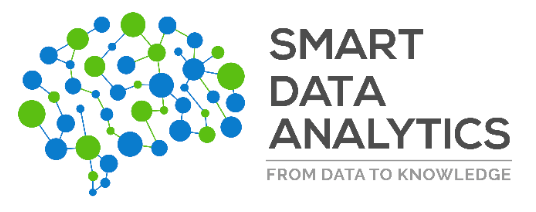
\includegraphics[width=0.45\textwidth]{material/crop-cooperation-sda.png}\\

	
\includegraphics[width=0.45\textwidth]{material/crop-cooperation-ssb.png}\\

	% Statistics Norway
	% Institute for Numerical Simulation
  
\includegraphics[width=0.45\textwidth]{material/crop-cooperation-limes.png}\\
	\vspace{1.75cm}
  
\includegraphics[width=0.45\textwidth]{material/crop-cooperation-lausanne.png} \\

  \column{.5\textwidth}
  \centering \\

\end{columns}

\end{frame}
%-------------------------------------------------------------------------------
%-------------------------------------------------------------------------------
